
\documentclass[11pt,a4paper]{article}

\usepackage{parskip}
\usepackage[utf8]{inputenc}
\usepackage{amsmath, amssymb, amsthm}
\usepackage{graphicx}
\usepackage{hyperref}
\usepackage{geometry}
\geometry{margin=1in}
\usepackage{enumitem}
\usepackage{mlmodern}

\title{Random Graph Generation}
\author{Santiago López Pereyra}
\date{}

\begin{document}

\maketitle

\section*{Introduction}

The generation of connected random graphs is non-trivial and important to many
applications. In general, given $n, m \in \mathbb{N}$, it is not difficult to
sample a random graph from the space of all graphs of $n$ vertices, $m$ edges.
The problem becomes more difficult when we require (a) that the randomly
generated graph be \emph{connected} and, if possible, (b) that any possible such graph
has the same probability of being generated (i.e. that we sample the connected
graphs with uniformity).


\begin{figure}[h!]
\centering
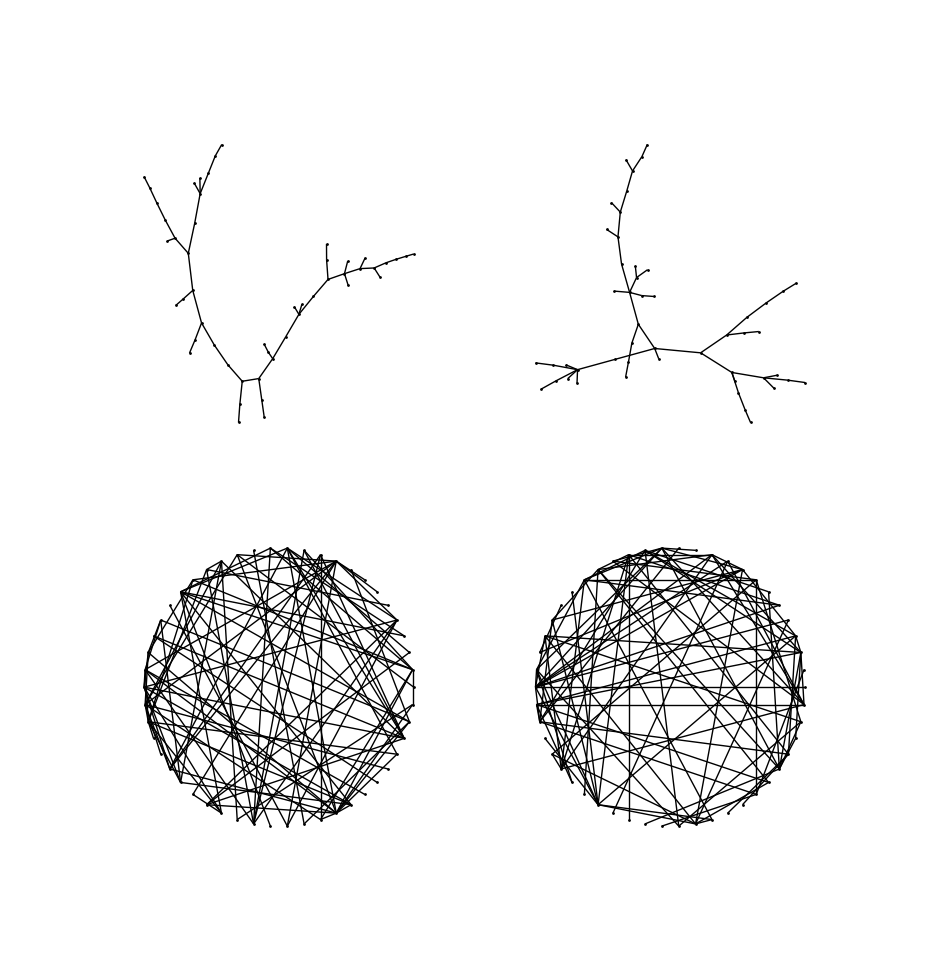
\includegraphics[width=0.85\textwidth]{../Images/RandGraphs.png}
\caption{Randomly generated graphs}
\end{figure}

A direct and simple algorithm is to generate a random tree (e.g. via a Prufer
sequence) and add edges randomly until the desired number of edges is reached.  
This procedure is relatively efficient ($\mathcal{O}(n^2)$), but it is biased.
Not all connected graphs have the same number of spanning trees, and
therefore the probability of generating a given connected graph is not uniform.

A computationally heavier approach is to generate a $K_n$ and prune edges
randomly until the desired number of edges is reached, while maintaining the 
connecitivity invariant. This algorithm is unbiased, but its complexity is
higher. The procedure is as follows:

\[
\begin{aligned}
&(V, E) := \textbf{genKn}(n)\\
&E_c := [e_1, \ldots, e_{|E|}]\\
&\textbf{while } |E| > m  \textbf{ do}\\
&\quad \left\{ v, w \right\}  := \textbf{randSample}(E_c)\\
&\quad E := E - \{v, w\}\\[4pt]
&\quad \textbf{if } \neg \textbf{ConnectivityCheck}(E, v, w) \textbf{ then}\\
&\quad\quad E := E \cup \{v, w\}\\
&\quad\quad E_c := E_c - \{v, w\} \quad \text{// edge is a bridge}\\
&\quad \textbf{fi}\\
&\textbf{od}\\[4pt]
&\textbf{return } (V, E)
\end{aligned}
\]

Generating a $K_n$ is $O(n^2)$. The $\textbf{while}$ selects a random edge
from $E_c$ and attempts to prune it. There is only one case in
which an edge is not removed; namely, when the sampled edge is a bridge. This
happens at most once per bridge. There are at most $n - 1$ bridges in a graph.
Hence, there are $O(n)$ iterations which do not remove an edge.

The remaining iterations will remove an edge and there will be exactly
$\frac{n(n-1)}{2} - m$ of them.

$\therefore$ There are $O(n) + O(\frac{n(n-1)}{2} - m) = O(n^2 - m)$
iterations.

The operations in each iteration are $O(1)$ except the connectivity check, which
we assume to be a BFS search with starting vertex $v$ and target vertex $w$. BFS
is $O(n^2)$.

$\therefore$ The algorithm is $O(n^2) + O(n^2 - m)O(n^2) = O(n^4 - n^2m)$.

In practice the algorithm will perform better than this. BFS stops whenever $w$
is found starting from $v$. This still is asymptotically $O(|E|)$, but in
practice the bound will seldom be reached. Furthermore, BFS is ran on
increasingly sparser graphs. Its asymptotic complexity is given by the number of
edges in the initial $K_n$, but it decreases with each pruning iteration.

To prove that the algorithm is unbiased we need a few definitions. Let
$\mathcal{G}_{n,m}$ denote the set of all graphs with $n$ vertices and $m$
edges, and let $\mathcal{C}_{n,m} \subset \mathcal{G}_{n,m}$ denote the subset
of \emph{connected} graphs. 

Let $\mathcal{E}_{n,m}$ be the class of edge sets $W \subseteq E(K_n)$ such that
removing $W$ from $K_n$ produces a connected graph with $m$ edges. 
Each $G \in \mathcal{C}_{n,m}$ corresponds uniquely to one such $W \in
\mathcal{E}_{n,m}$, so
\[
    |\mathcal{E}_{n,m}| = \left| \mathcal{C}_{n, m}\right| .
\]
It follows that there is a bijection
\[
f_{n,m} : \mathcal{E}_{n,m} \to \mathcal{C}_{n,m},
\quad
f_{n,m}(W) = (V, E( K_n ) - W).
\]

We now prove that:
\begin{enumerate}
    \item[(1)] The edges removed by the algorithm form a valid set $W \in
        \mathcal{E}_{n,m}$ and the resulting graph is $f_{n,m}(W)$.
    \item[(2)] Each $W \in \mathcal{E}_{n,m}$ may be formed with equal probability.
\end{enumerate}

\paragraph{(1)}
The algorithm removes $k = \binom{n}{2} - m$ edges $S = \left\{ e_1, \ldots, e_k
\right\} $. The
connectivity invariant is preserved at each successful removal, so 
$\left\{ e_1 \right\}, \left\{ e_1, e_2 \right\}, \ldots, \left\{ e_1, \ldots,
e_k \right\}   $ are all members of $\mathcal{E}_{n, m}$. By construction, the
final graph has edges $E(K_n) - S$, i.e. the final graph equals \(f_{n,m}(S)\).
$\blacksquare$

\paragraph{(2) Unbiasedness (symmetry argument)}
The algorithm removes the edges of some \(W \in \mathcal{E}_{n,m}\) and each
successful run corresponds to an ordered sequence \((e_1,\dots,e_k)\) which is a
permutation of the elements of that \(W\). Note that:

\begin{enumerate}
  \item If \(W\in\mathcal{E}_{n,m}\), then for any subset \(S'\subseteq W\)
  the graph \(f(S')\) is still connected (removing fewer edges
  cannot disconnect a graph that remains connected after removing the larger set).
  Hence any permutation of the \(k\) edges of \(W\) is an admissible removal
  order: none of those edges will ever be a bridge at the moment it is
  removed. Therefore the number of admissible orders that produce \(W\) is
  exactly \(k!\).
  \item By vertex- and edge-symmetry of \(K_n\), the size \(|E_i|\) of the
  candidate set at step \(i\) depends only on \(i\) (and on \(n,m\)), not on
  which particular edges form \(S_{i-1}\). Denote \(a_i:=|E_i|\).
\end{enumerate}


At step \(i\) the algorithm chooses uniformly from \(E_i\), so the probability
of that exact ordered sequence is \(\prod_{i=1}^k \frac{1}{a_i}\). Since there
are \(k!\) ordered sequences (permutations) that yield the same unordered set
\(W\), the probability of producing \(W\) equals
\[
\Pr[\text{output } W] \;=\; k! \prod_{i=1}^k \frac{1}{a_i}.
\]
The right-hand side does not depend on \(W\) (only on \(k\) and the
sequence \(a_i\)), so every \(W\in\mathcal{E}_{n,m}\) is produced with the
same probability. Thus the induced distribution on \(\mathcal{C}_{n,m}\) is
uniform, i.e.\ the algorithm is unbiased.


\begin{figure}[h!]
\centering
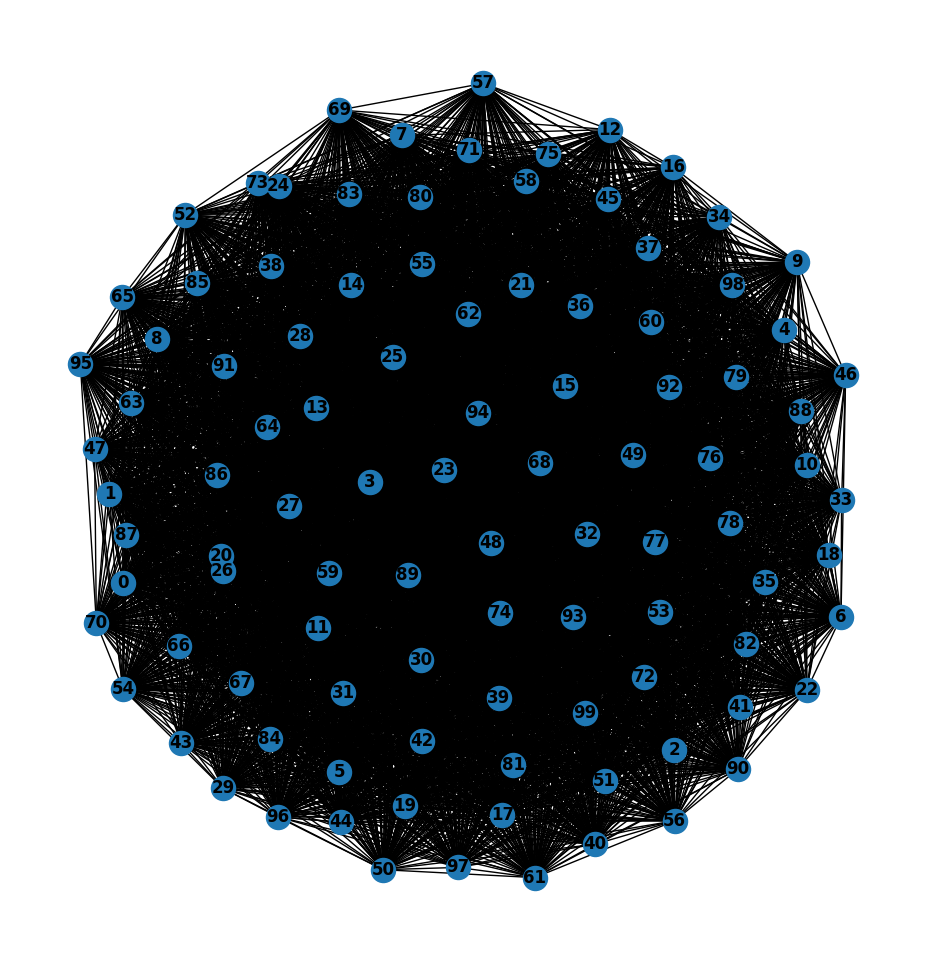
\includegraphics[width=0.45\textwidth]{../Images/K100.png}
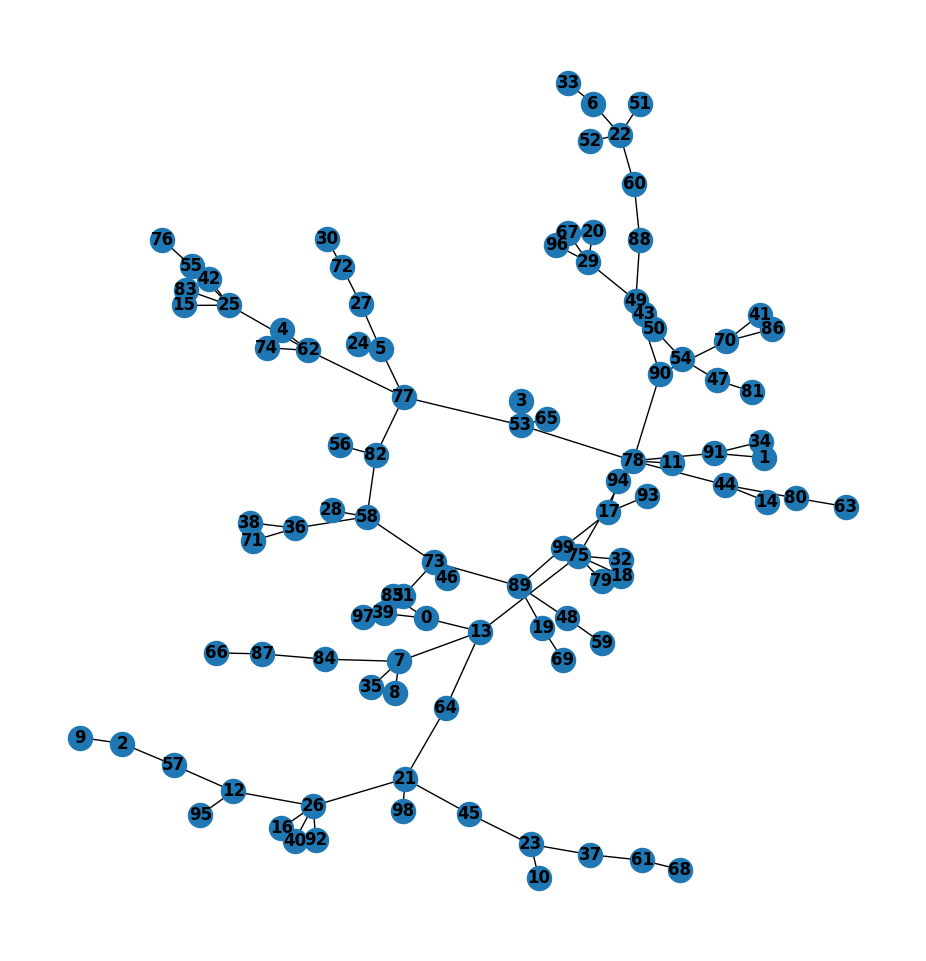
\includegraphics[width=0.45\textwidth]{../Images/TreeFromK100.png}
\caption{A complete graph $K_{100}$ (left) and a random tree obtained by pruning (right).}
\end{figure}

\section{As a Markov chain}

Let $G_i$ denote the graph after $i$ successful iterations of the edge-pruning algorithm. Then the sequence $\{G_i\}_{i\ge 0}$ defines a discrete-time Markov chain (DTMC) on the state space $\mathcal{C}_{n,m}$, the set of connected graphs with $n$ vertices and $m$ edges.  

\subsection*{Markov property}

The Markov property holds because the choice of edge to remove at step $i+1$ depends solely on the current graph $G_i$ and the remaining candidate edges $E_c$. Formally, for all $i\ge 0$ and all $G_0, \dots, G_{i+1} \in \mathcal{C}_{n,m}$,
\[
\Pr[G_{i+1} \mid G_i, G_{i-1}, \dots, G_0] = \Pr[G_{i+1} \mid G_i].
\]

\subsection*{Transition probabilities}

Let $P(G_i \to G_{i+1})$ denote the one-step transition probability from graph
$G_i$ to graph $G_{i+1}$, assuming $G_{i+1} \neq G_i$. Then
\[
P(G_i \to G_{i+1}) =
\begin{cases}
    \frac{1}{|E_i|}, & \text{if $G_{i+1}$ can be obtained by removing a single
    non-bridge edge from $G_i$,} \\
0, & \text{otherwise,}
\end{cases}
\]
If a sampled edge is a bridge, then the graph remains unchanged and $G_i =
G_{i+1}$. The probability of this self-loop transition is given by
\[
P(G_i \to G_i) = \frac{|B_i|}{m_i},
\]
where $B_i$ is the set of bridge edges at the current iteration and $m_i$ is
number of edges in $G_i$. Note that $B_i = \overline{E_i}$, which means 
$\left| B_i \right| = m_i - \left| E_i \right| $, entailing that

\begin{equation*}
P(G \to G) = \frac{m_i - \left| E_i \right| }{m_i} = 1 - \frac{\left| E_i
\right| }{m_i} 
\end{equation*}

From this follows that the probability that an edge is successfully removed at 
iteration $i$ is $\left| E_i \right| / m_i$. 

Note that there are at most $n-1$ bridges in a connected graph with $n$
vertices, and this bound remains constant across iterations, so at any given
point in time we have 

\begin{equation*}
     P(\text{A bridge is chosen at iteration } i) \leq \frac{n-1}{m_i}
\end{equation*} 

Obviously, this bound is informative only when $m_i \gg n - 1$, since otherwise
the bound approximates $1$ and becomes trivial. This of course means that the
bound is informative for dense graphs and not for sparse ones.

\subsection*{Stationary distribution}

Since the algorithm is unbiased, every connected graph $G \in \mathcal{C}_{n,m}$ is equally likely to appear as the final output. This implies that the stationary distribution $\pi$ of the Markov chain is uniform over $\mathcal{C}_{n,m}$:
\[
\pi(G) = \frac{1}{|\mathcal{C}_{n,m}|}, \quad \forall G \in \mathcal{C}_{n,m}.
\]

\subsection*{Irreducibility and aperiodicity}

The chain is irreducible in the sense that, starting from $K_n$, any connected graph with $m$ edges can eventually be reached by a sequence of valid edge removals.  
The chain is aperiodic because there is a positive probability of staying in the same state (when a bridge is sampled), i.e.,
\[
P(G \to G) > 0 \quad \forall G \in \mathcal{C}_{n,m}.
\]
Hence, the Markov chain converges to the uniform stationary distribution.




\section{An improvement}

The probability that a chosen edge is a bridge increases as the graph becomes
sparser, but is relatively negligible in the early stages of the algorithm.
Since such probability is bounded at each iteration by $n-1 / m_i$, and both of
these quantities are known to the algorithm, we can define a tolerance $\epsilon$
s.t. if $n-1 / m_i < \epsilon$, we skip the connectivity check and
automatically remove the sampled edge. 
















\end{document}
